%% Preamble %%
%% A minimal LaTeX preamble
%% Some packates are needed to implement
%% Asciidoc features

\documentclass[11pt,twocolumn,oneside]{article}
\setlength{\columnsep}{1cm}
%\setlength{\columnseprule}{thickness}
\usepackage[brazilian]{babel}
\usepackage[a4paper,
            %bindingoffset=0.2in,%
            left=3cm,right=3cm,top=3cm,bottom=3cm,%
            %footskip=.25in
            ]
            {geometry}
\usepackage[figurename=Fig.,font=footnotesize,labelfont=bf]{caption}
\usepackage{fancyhdr}

\pagestyle{fancy}
%\fancyhf{}
%\rhead{Overleaf}
%\lhead{Guides and tutorials}
\lfoot{\tiny{Prof. Jefferson Oliveira}}
%\cfoot{}
%\rfoot{\thepage}
%\usepackage{geometry}                % See geometry.pdf to learn the layout options. There are lots.
%\geometry{a4paper}               % ... or a4paper or a5paper or ...
%\geometry{landscape}                % Activate for for rotated page geometry
%\usepackage[parfill]{parskip}       % Activate to begin paragraphs with an empty line rather than an indent

\usepackage{tcolorbox}
\usepackage{lipsum}

\usepackage{epstopdf}
\usepackage{color}
% \usepackage[usenames, dvipsnames]{color}
% \usepackage{alltt}


\usepackage{amssymb}
% \usepackage{amsmath}
\usepackage{amsthm}
\usepackage[version=3]{mhchem}


% Needed to properly typeset
% standard unicode characters:
%
\RequirePackage{fix-cm}
\usepackage{fontspec}
\usepackage[Latin,Greek]{ucharclasses}
%
% NOTE: you must also use xelatex
% as the typesetting engine


% \usepackage{fontspec}
% \usepackage{polyglossia}
% \setmainlanguage{en}

\usepackage{hyperref}
\hypersetup{
    colorlinks=true,
    linkcolor=blue,
    filecolor=magenta,
    urlcolor=cyan,
}

\usepackage{graphicx}
\usepackage{wrapfig}
\graphicspath{ {images/} }
\DeclareGraphicsExtensions{.png, .jpg, jpeg, .pdf}

%% \DeclareGraphicsRule{.tif}{png}{.png}{`convert #1 `dirname #1`/`basename #1 .tif`.png}
%% Asciidoc TeX Macros %%


% \pagecolor{black}
%%%%%%%%%%%%


% Needed for Asciidoc

\newcommand{\admonition}[2]{\textbf{#1}: {#2}}
\newcommand{\rolered}[1]{ \textcolor{red}{#1} }
\newcommand{\roleblue}[1]{ \textcolor{blue}{#1} }

\newtheorem{theorem}{Theorem}
\newtheorem{proposition}{Proposition}
\newtheorem{corollary}{Corollary}
\newtheorem{lemma}{Lemma}
\newtheorem{definition}{Definition}
\newtheorem{conjecture}{Conjecture}
\newtheorem{problem}{Problem}
\newtheorem{exercise}{Exercise}
\newtheorem{example}{Example}
\newtheorem{note}{Note}
\newtheorem{joke}{Joke}
\newtheorem{objection}{Objection}





%%%%%%%%%%%%%%%%%%%%%%%%%%%%%%%%%%%%%%%%%%%%%%%%%%%%%%%

%  Extended quote environment with author

\renewenvironment{quotation}
{   \leftskip 4em \begin{em} }
{\end{em}\par }

\def\signed#1{{\leavevmode\unskip\nobreak\hfil\penalty50\hskip2em
  \hbox{}\nobreak\hfil\raise-3pt\hbox{(#1)}%
  \parfillskip=0pt \finalhyphendemerits=0 \endgraf}}


\newsavebox\mybox

\newenvironment{aquote}[1]
  {\savebox\mybox{#1}\begin{quotation}}
  {\signed{\usebox\mybox}\end{quotation}}

\newenvironment{tquote}[1]
  {  {\bf #1} \begin{quotation} \\ }
  { \end{quotation} }

%% BOXES: http://tex.stackexchange.com/questions/83930/what-are-the-different-kinds-of-boxes-in-latex
%% ENVIRONMENTS: https://www.sharelatex.com/learn/Environments

\newenvironment{asciidocbox}
  {\leftskip6em\rightskip6em\par}
  {\par}

\newenvironment{titledasciidocbox}[1]
  {\leftskip6em\rightskip6em\par{\bf #1}\vskip-0.6em\par}
  {\par}



%%%%%%%%%%%%%%%%%%%%%%%%%%%%%%%%%%%%%%%%%%%%%%%%%%%%%%%%

%% http://texblog.org/tag/rightskip/


\newenvironment{preamble}
  {}
  {}

%% http://tex.stackexchange.com/questions/99809/box-or-sidebar-for-additional-text
%%
\newenvironment{sidebar}[1][r]
  {\wrapfigure{#1}{0.5\textwidth}\tcolorbox}
  {\endtcolorbox\endwrapfigure}


%%%%%%%%%%

\newenvironment{comment*}
  {\leftskip6em\rightskip6em\par}
  {\par}

  \newenvironment{remark*}
  {\leftskip6em\rightskip6em\par}
  {\par}


%% Dummy environment for testing:

\newenvironment{foo}
  {\bf Foo.\ }
  {}


\newenvironment{foo*}
  {\bf Foo.\ }
  {}


\newenvironment{click}
  {\bf Click.\ }
  {}

\newenvironment{click*}
  {\bf Click.\ }
  {}  
  
\newenvironment{resposta*}
  {\bf Resposta:\\ }
  {}

\newenvironment{resposta}
  {\bf Resposta:\\ }
  {}  
  
\newenvironment{remark}
  {\bf Remark.\ }
  {}

\newenvironment{capsule}
  {\leftskip10em\par}
  {\par}

%%%%%%%%%%%%%%%%%%%%%%%%%%%%%%%%%%%%%%%%%%%%%%%%%%%%%

%% Style

\parindent0pt
\parskip8pt
%% User Macros %%
%% Front Matter %%

\title{Fundamentos da Óptica Geométrica}
\author{Jefferson Rodrigues de Oliveira}
\date{10-11-2020}


%% Begin Document %%

\begin{document}
\maketitle
\tableofcontents
\hypertarget{x-objetivos}{\section{Objetivos}}
Caro aluno, logo abaixo apresentarei \textbf{os principais objetivos que você deve alcançar} ao estudar este conteúdo:


\begin{itemize}

\item \textbf{Compreender} que a luz em um meio uniforme desloca em linha reta e com velocidade finita.

\item \textbf{Saber explicar} como as sombras são formadas.

\item \textbf{Saber explicar} como objetos não luminosos podem ser vistos.

\item \textbf{Conhecer} os efeitos dos filtros na luz branca.

\item \textbf{Compreender} como objetos coloridos aparecem sob a luz branca e outras cores.

\end{itemize}


\hypertarget{x-raios-de-luz-e-feixes-de-luz}{\section{Raios de luz e feixes de luz}}
A Óptica Geométrica estuda a \textbf{propagação da luz} nos diferentes meios e os fenômenos que dela decorrem: a \textbf{reflexão} e a \textbf{refração}. Este estudo é feito a partir da noção de \textbf{raio de luz} e de \textbf{princípios fundamentais}.


Ondas de rádio, micro-ondas, radiações infravermelha e ultravioleta, luz, raios X, etc. São constituintes das chamadas \textbf{ondas eletromagnéticas}. A luz difere das demais ondas pelo fato de, ao incidir em nossas vidas, produzir as \textbf{sensações visuais}. Ou seja, a \textbf{luz} é o agente físico que, atuando nos órgãos visuais, é capaz de produzir a \textbf{sensação de visão}.


Para que um observador possa enxergar um corpo, seus olhos devem receber a luz que este corpo emite.


Para representar a luz emitida pela chama de uma vela que atinge a vista de um observador, utilizaremos linhas orientadas que fornecem a direção e o sentido de propagação da luz. Tais linhas são denominadas \textbf{raios de luz}.


\begin{figure}[h]{}
\centering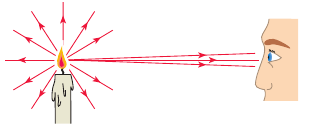
\includegraphics[width=2.5truein]{img0.png}
\caption{Raios de luz que chegam no observador. Fonte: Os Fundamentos da Física. Vol 2.}
\centering
\end{figure}

Na prática, é impossível isolar um raio de luz, que, na verdade, é apenas uma representação gráfica da luz em propagação. O que realmente existe são os chamados \textbf{feixes de luz}, que representamos graficamente como um conjunto de raios de luz. Os feixes de luz podem ser:


\begin{itemize}

\item \textbf{Cilíndricos}: os raios de luz são paralelos entre si.

\end{itemize}


\begin{figure}[h]{}
\centering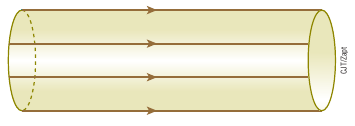
\includegraphics[width=2.5truein]{img3.png}
\caption{Feixe cilíndrico. Fonte: Tópicos de Física. Vol 2.}
\centering
\end{figure}

\begin{itemize}

\item \textbf{Cônicos divergentes}: os raios de luz divergem de um mesmo ponto \textbf{P}.

\end{itemize}


\begin{figure}[h]{}
\centering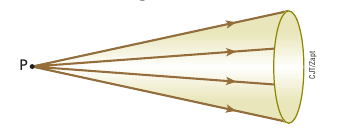
\includegraphics[width=2.5truein]{img1.png}
\caption{Feixe cônico divergente. Fonte: Tópicos de Física. Vol 2.}
\centering
\end{figure}

\begin{itemize}

\item \textbf{Cônicos convergentes}: os raios de luz convergem para um mesmo ponto \textbf{P}.

\end{itemize}


\begin{figure}[h]{}
\centering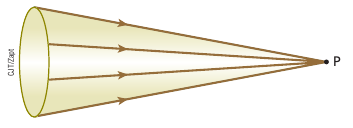
\includegraphics[width=2.5truein]{img2.png}
\caption{Feixe cônico convergente. Fonte: Tópicos de Física. Vol 2.}
\centering
\end{figure}

\hypertarget{x-fontes-de-luz}{\section{Fontes de luz}}
Todos os corpos que emitem luz são chamados de \textbf{fontes de luz}.


Podemos classificar estas fontes de acordo com a \textbf{emissão da luz}.


\begin{itemize}

\item \textbf{Fonte de luz primária (corpo luminoso)}: corpos que emitem a luz que eles produzem, ou seja, \textbf{emitem luz própria}. Exemplo: Sol, lâmpada elétrica acesa, chamas das velas, etc.

\item \textbf{Fonte de luz secundária (corpo iluminado)}: corpos que emitem a luz que recebem de outros corpos, ou seja \textbf{não produzem luz própria}. Exemplo: a Lua, que envia à Terra a luz que recebe do Sol, das paredes iluminadas por uma lâmpada elétrica, etc.

\end{itemize}


Podemos também classificar estas fontes de acordo com suas \textbf{dimensões}:


\begin{itemize}

\item \textbf{Fonte de luz pontual (puntiforme)}: são fontes cujas dimensões são desprezíveis em relação à distância que a separam dos outros corpos. Exemplo: A maioria das estrelas, apesar delas serem enormes, as distância que as separam do nosso planeta são muito maiores.

\item \textbf{Fonte de luz extensa}: são fontes cujas dimensões \textbf{não} são desprezíveis em relação à distância que a separam dos outros corpos. Exemplo: O Sol, observado da Terra.

\end{itemize}


Por fim, também podemos classificar estas fontes de acordo com suas cores:


\begin{itemize}

\item \textbf{Fonte de luz monocromática (simples)}: fonte de luz que apresentam apenas uma cor. Exemplo: a luz amarela emitida por lâmpadas de vapor de sódio.

\item \textbf{Fonte de luz policromática (composta)}: fonte de luz que resulta da superposição de luzes de cores diferentes. Exemplo: a luz solar (branca).

\end{itemize}


\hypertarget{x-velocidade-da-luz}{\subsection{Velocidade da luz}}
A velocidade da luz no vácuo é de $299792458\;m/s$, ou seja, aproximadamente $3,0\times 10^{8}\;m/s$. No \textbf{vácuo}, a luz apresenta \textbf{máxima velocidade}, independente da cor, ou seja, todas as cores apresentam a mesma velocidade igual a $c$. Entretanto, em meios materiais, as luzes monocromáticas apresentam velocidades diferentes, todas inferiores a $c$.


\hypertarget{x-ano-luz}{\subsection{Ano-luz}}
\textbf{Ano-luz} é a unidade de \textbf{comprimento} que corresponde à distância percorrida pela luz, no vácuo, durante um ano.


Para se ter uma ideia da dimensão do ano-luz, vamos transformá-lo em metros e depois em quilômetros. Imagine que no instante $t=0$ um novo raio de luz partiu do Sol e vai para o "infinito". Vamos acompanhá-lo durante 1 ano e medir a distância percorrida.
\begin{align*}
    1\;ano  &= 365,25\;dias \\
            &= 8776\;horas \\
            &= 525960\;min \\
            &= 31557600\;s \\
            &\approx 3,16\times 10^{7}\;s
\end{align*}
Utilizando a fórmula da velocidade média:
\begin{align*}
    v &= \dfrac{\Delta S}{\Delta t} \\
    c &= \dfrac{d}{t} \\
    d &= c \cdot t \\
    d &= 3,0\times 10^{8} \cdot 3,16\times 10^{7} \\
    d &\approx 9,5 \times 10^{15}
\end{align*}
Sendo assim, a velocidade da luz no vácuo é de aproximadamente $9,5\times 10^{15}\;m$ ou $9,5\times 10^{12}\;km$.


Esta unidade é bastante utilizada na \textbf{Astronomia}, devido às distância das estrelas até o nosso planeta.


\hypertarget{x-classificação-dos-meios}{\section{Classificação dos meios}}
\begin{itemize}

\item \textbf{Meios transparentes} são aqueles que permitem que a luz os atravesse descrevendo \textbf{trajetórias regulares e bem definidas}, ou seja, quando a luz atravessa o meio  e \textbf{permite} a visualização nítida dos objetos. O único meio absolutamente transparente é o vácuo, todavia, também podem ser considerados transparentes o ar atmosférico, a água pura, entre outros.

\end{itemize}


\begin{figure}[h]{}
\centering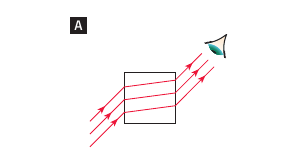
\includegraphics[width=2.5truein]{img4.png}
\caption{Meio transparente. Fonte: Os Fundamentos da Física. Vol 2.}
\centering
\end{figure}

\begin{itemize}

\item \textbf{Meios translúcidos} são aqueles em que a luz descreve \textbf{trajetórias irregulares com intensa difusão (espelhamento aleatório)}, provocada pelas partículas deste meio, ou seja, quando a luz atravessa o meio e \textbf{não permite} uma visão nítida dos objetos. É o que ocorre, por exemplo, quando a luz atravessa a neblina, o papel-manteiga, entre outros.

\end{itemize}


\begin{figure}[h]{}
\centering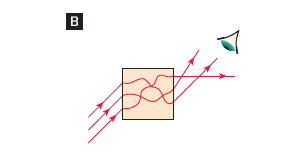
\includegraphics[width=2.5truein]{img5.png}
\caption{Meio translúcido. Fonte: Os Fundamentos da Física. Vol 2.}
\centering
\end{figure}

\begin{itemize}

\item \textbf{Meios opacos} são aqueles através dos quais \textbf{a luz não se propaga}. Depois de incidir em um meio opaco, a luz é parcialmente absorvida e parcialmente refletida pelo meio. São opacos os seguinte meios: madeira, alvenaria, metais, entre outros.

\end{itemize}


\begin{figure}[h]{}
\centering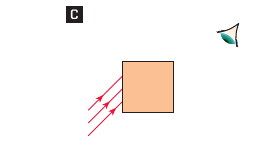
\includegraphics[width=2.5truein]{img6.png}
\caption{Meio opaco. Fonte: Os Fundamentos da Física. Vol 2.}
\centering
\end{figure}

Um meio em que todos os seus elementos de volume possuem as mesmas propriedades é denominado \textbf{homogêneo}. O vácuo é um meio homogêneo por excelência. O ar, em pequenas quantidades, pode ser considerado homogêneo. Mas a atmosfera com um todo não é homogênea.


Quando as associadas a um elemento de volume independem da direção, o meio é chamado de \textbf{isotrópico}. Por exemplo, em um cristal cúbico, a velocidade da luz é igual qualquer que seja a direção em que é medida, caracterizando assim um meio isotrópico. Meios que simultaneamente são homogêneos e isotrópicos são denominados de \textbf{ordinários}.


\textbf{Exercício Resolvido 1}


\textbf{(FUVEST SP)} Admita que o Sol subitamente "morresse", ou seja, sua luz deixasse de ser emitida. Vinte e quatro horas após esse evento, um eventual sobrevivente, olhando para o céu, sem nuvens, veria:


a)	a Lua e estrelas; \\
b)	somente a Lua; \\
c)	somente estrelas; \\
d)	uma completa escuridão; \\
e)	somente os planetas do sistema solar.


\begin{resposta*}
{\it Após $24\;h$, não conseguiríamos observar o Sol e nem a Lua (corpo ilumindo pelo Sol). Portanto, apenas conseguiríamos observar as estrelas. \\
\textbf{Resposta: c.}}
\end{resposta*}

\textbf{Exercício Resolvido 2}


Um ano-luz tem a dimensão de:


a) tempo; \\
b) velocidade; \\
c) aceleração; \\
d) comprimento; \\
e) energia.


\begin{resposta*}
{\it Um \textbf{ano-luz} é a distância que a luz percorre no vácuo durante um ano terrestre. A dimensão de ano-luz é \textbf{comprimento}. \\
\textbf{Resposta: d.}}
\end{resposta*}

\textbf{Exercício Resolvido 3}


Uma estrela está situada a $4\;anos-luz$ da Terra. Qual a distância entre a estrela e a Terra em quilômetros?


\begin{resposta*}
{\it $1\;ano-luz$ corresponde aproximadamente a $9,5\times 10^{12}\;km$. Portanto, $4\;anos-luz$ correspondem a $4\cdot 9,5\times 10^{12}\;km = 3,8\times 10^{13}\;km$.}
\end{resposta*}

\textbf{Exercício Resolvido 4}


Marque \textbf{V} para o item verdadeiro e \textbf{F} para o item falso:


a) O ar atmosférico de uma sala é um meio transparente. \\
b) A água em camadas espessas é um meio transparente. \\
c) O vidro fosco é um meio translúcido. \\
d) A atmosfera terrestre, cuja densidade diminui com o aumento da altitude, é um meio homogêneo. \\
e) Nos meios transparentes e translúcidos a luz se propaga em linha reta.


\begin{resposta*}
{\it a) \textbf{Verdadeiro}. O ar atmosférico existente em uma sala é um meio transparente. \\
b) \textbf{Falso}. A água em pequenas camadas e um meio transparente. Já em camadas espessas não é um meio transparente. \\
c) \textbf{Verdadeiro}. Através do vidro fosco os objetos não são vistos nitidamente. Logo é um meio translúcido. \\
d) \textbf{Falso}. Um meio homogêneo apresenta as mesmas propriedades em todos os seus pontos. \\
e) \textbf{Falso}. A luz se propaga em linha reta nos meios transparentes e homogêneos.}
\end{resposta*}

\textbf{Exercício de Revisão 1}


\textbf{(ITA SP)} Dos objetos citados a seguir, assinale aquele que seria visível em uma sala perfeitamente escura:


a)	um espelho; \\
b)	qualquer superfície de cor clara; \\
c)	um fio aquecido ao rubro; \\
d)	uma lâmpada desligada; \\
e)	um gato preto.


\begin{resposta*}
{\it \textbf{c}.}
\end{resposta*}

\textbf{Exercício de Revisão 2}


\textbf{(IBFC/2016)} O feixe de luz é um ente que não tem existência real. Seu comportamento pode assumir diferentes formas ao atravessar ou não alguns materiais. Considere as seguintes afirmativas sobre o comportamento da luz com relação aos meios:


I - No meio transparente, a luz é refletida no sentido contrário de sua origem, como em um espelho. \\
II - No meio translúcido, a luz se propaga de forma irregular, de modo que o observador vê o objeto através do meio, mas sem nitidez, como o papel vegetal. \\
III - No meio opaco, a luz não se propaga, não sendo possível ao observador ver o objeto atrás, como uma cortina. \\
Estão corretas as afirmativas:


a) II, III. \\
b) I, II. \\
c) I, II, III. \\
d) I, III. \\
e) somente III.


\begin{resposta*}
{\it \textbf{a}.}
\end{resposta*}

\textbf{Exercício de Revisão 3}


\textbf{(PUC MG/2014)} Certa estrela emite luz que percorre a distância de um bilhão de anos-luz até chegar à Terra e ser captada por um telescópio. É CORRETO afirmar:


a)	A estrela está a uma distância de um bilhão de quilômetros da Terra. \\
b)	Daqui a um bilhão de anos, a luz dessa estrela não mais chegará à Terra. \\
c)	A luz recebida hoje aqui na Terra foi emitida há um bilhão de anos. \\
d)	Quando a luz foi emitida pela estrela, ela tinha a idade de um bilhão de anos.


\begin{resposta*}
{\it \textbf{c}.}
\end{resposta*}

\textbf{Exercício de Revisão 4}


\textbf{(FUVEST)} No mês de agosto de 1988, o planeta Marte teve a máxima aproximação da Terra. Nesse dia as pessoas, ao observarem o planeta, estavam vendo a luz emitida pelo Sol algum tempo antes. Aproximadamente quanto tempo antes? Considere as órbitas da Terra e de Marte circulares e coplanares, com raios de $150.000.000\;km$ e $231.000.000\;km$, respectivamente. \\
Dado: velocidade da luz: $300.000\;km/s$.


a) $81\;anos-luz$ \\
b) $2\;horas$ \\
c) $30\;segundos$ \\
d) $8\;minutos$ \\
e) 17 minutos


\begin{resposta*}
{\it \textbf{e}.}
\end{resposta*}

\hypertarget{x-fenômenos-da-óptica-geométrica}{\section{Fenômenos da Óptica Geométrica}}
A óptica geométrica estuda, basicamente, trajetórias de luz em sua propagação. São de especial interesse nesse estudo dois fenômenos físicos fundamentais: a \textbf{reflexão} e a \textbf{refração}.


\begin{itemize}

\item \textbf{Reflexão} é o fenômeno que consiste no fato de a luz voltar a se propagar no meio de origem, após incidir na superfície de separação deste com outro meio.

\item \textbf{Refração} é o fenômeno que consiste no fato de a luz passar de um meio para outro diferente.

\end{itemize}


\begin{figure}[h]{}
\centering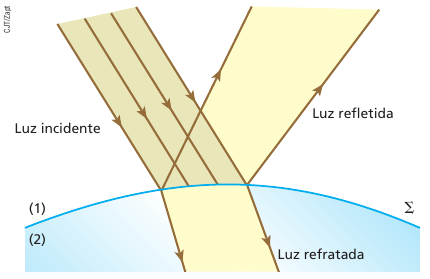
\includegraphics[width=2.5truein]{img7.png}
\caption{Luz incidente, refletida e refratada. Fonte: Tópicos de Física. Vol 2.}
\centering
\end{figure}

De acordo com a regularidade da superfície que a luz incide, pode-se determinar dois tipos de reflexão e refração: \textbf{regular} e \textbf{difusa}.


Para entender melhor esses dois tipos de reflexão e refração, vamos pensar em suas situações:


\begin{enumerate}

\item{Superfície da água de um lago isenta de qualquer tipo de perturbação.}

\item{Superfície da água de um lago perturbado por gotas de chuva.}

\end{enumerate}


Na primeira situação, observa-se que após a incidência da luz na água, tanto o feixe de luz refletido quanto o refratado \textbf{são de forma cilíndrica}, ou seja, os raios são paralelos entre si. Essa situação caracteriza a reflexão e refração \textbf{regular}. Este tipo de reflexão e refração ocorrem em \textbf{superfícies perfeitamente lisas}.


\begin{figure}[h]{}
\centering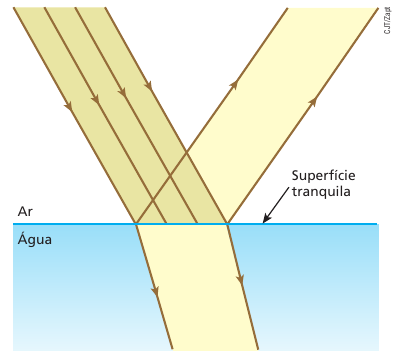
\includegraphics[width=2.5truein]{img8.png}
\caption{Reflexão e Refração regular. Fonte: Tópicos de Física. Vol 2.}
\centering
\end{figure}

Já na segunda situação, observa-se que após a incidência da luz na água, tanto o feixe de luz refletido quanto o refratado \textbf{não são de forma cilíndrica}, as componentes dos raios de luz possuem diversas direções e se espalham de forma aleatória. Essa situação caracteriza a reflexão e refração \textbf{difusa}. Este tipo de reflexão e refração ocorrem em \textbf{superfícies que possuem irregularidades}.


\begin{figure}[h]{}
\centering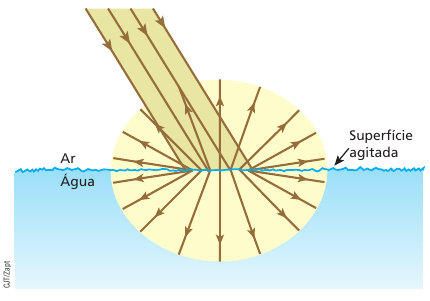
\includegraphics[width=2.5truein]{img9.png}
\caption{Reflexão e Refração difusa. Fonte: Tópicos de Física. Vol 2.}
\centering
\end{figure}

\hypertarget{x-a-cor-de-um-corpo}{\section{A cor de um corpo}}
A luz solar (ou a luz emitida por uma lâmpada fluorescente) é denominada \textbf{luz branca}.


A luz branca solar é \textbf{policromática}, ou seja, é composta por diversas cores, das quais podemos destacar sete: vermelho, alaranjado, amarelo, verde, azul, anil e violeta.


Por que quando iluminada pela luz do Sol, as folhas de uma árvore nos parecem verdes?


Porque essas folhas refletem de forma difusa para o meio a cor componente verde e absorvendo as demais cores componentes da luz branca.


\begin{figure}[h]{}
\centering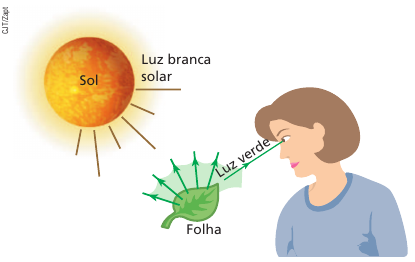
\includegraphics[width=2.5truein]{img10.png}
\caption{Cor de uma folha verde. Fonte: Tópicos de Física. Vol 2.}
\centering
\end{figure}

Vale ressaltar os seguintes pontos:


\begin{itemize}

\item Se vermos um corpo \textbf{branco,} é porque ele está \textbf{refletindo todas as cores} do espectro solar.

\end{itemize}


\begin{figure}[h]{}
\centering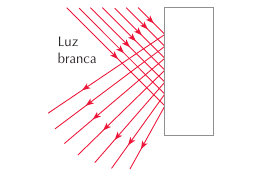
\includegraphics[width=2.5truein]{img11.png}
\caption{Corpo branco. Fonte: Os Fundamentos da Física. Vol 2.}
\centering
\end{figure}

\begin{itemize}

\item Se "vermos" um corpo \textbf{preto}, é porque ele está \textbf{absorvendo todas as cores} do espectro solar.

\end{itemize}


\begin{figure}[h]{}
\centering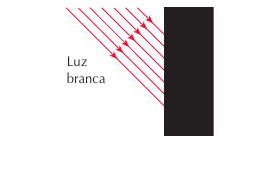
\includegraphics[width=2.5truein]{img12.png}
\caption{Corpo negro. Fonte: Os Fundamentos da Física. Vol 2.}
\centering
\end{figure}

\begin{itemize}

\item Um corpo que nos parece vermelho quando iluminado pela luz branca solar se apresentará escuro quando iluminado por luz monocromática de cor diferente da vermelha (azul, por exemplo).

\end{itemize}


Quando observamos um objeto através de uma lâmina de acrílico vermelha, por exemplo, apenas conseguiremos distinguir regiões vermelhas e escuras. Isto acorre porque a lâmina funciona como um \textbf{filtro}, que refrata (deixa passar) seletivamente a luz vermelha, absorvendo substancialmente as demais cores do espectro (regiões escuras).


\begin{figure}[h]{}
\centering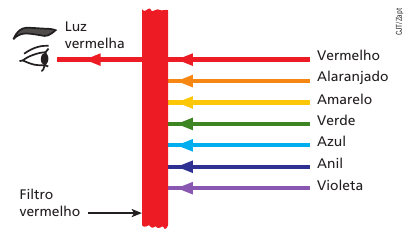
\includegraphics[width=2.5truein]{img13.png}
\caption{Esquema da refração seletiva. Fonte: Tópicos de Física. Vol 2.}
\centering
\end{figure}

\hypertarget{x-a-cor-do-céu}{\subsection{A cor do céu}}
Ao atravessar a atmosfera terrestre, a luz sofre difusão, isto é, espalhamento, de maneira mais acentuada na luz de cor \textbf{azul}.


Se não existe atmosfera, o céu seria sempre \textbf{negro}, exceto na direção do Sol. Este fato é notado, por exemplo, em grandes altitudes e na Lua (por não ter atmosfera).


As gotas de água que compõem as nuvens espalham, com a mesma intensidade, luzes de todas as cores. Por isto a nuvens são vistas \textbf{brancas}.


No nascer e por Sol, a luz atravessa uma espessura maior de atmosfera antes de atingir a atmosfera. Nessas condições, em virtude do maior espalhamento da luz azul e de cores próxima a ela, recebemos a luz subtraída destas cores, por este motivo, o Sol e o céu ao seu redor são vistos \textbf{avermelhados}.


\begin{figure}[h]{}
\centering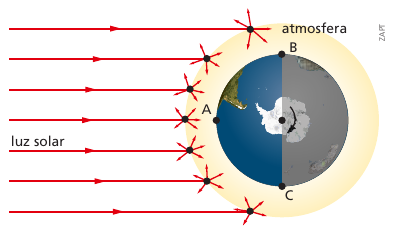
\includegraphics[width=2.5truein]{img14.png}
\caption{Cor do céu. Fonte: Física Clássica. Vol 2.}
\centering
\end{figure}

\hypertarget{x-princípios-da-ótica-geométrica}{\section{Princípios da Ótica Geométrica}}
Os princípios da Óptica Geométrica são:


\begin{itemize}

\item \textbf{Princípio da propagação retilínea}:

\end{itemize}


Nos meios homogêneos e transparentes, a luz se propaga em linha reta.


Este princípio constitui a base para a explicação de diversos fenômenos, como, por exemplo, a formação de sombras e penumbras.


\begin{figure}[h]{}
\centering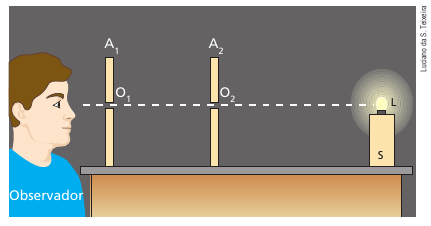
\includegraphics[width=2.5truein]{img15.png}
\caption{Propagação retilínea. Fonte: Tópicos de Física. Vol 2.}
\centering
\end{figure}

\begin{itemize}

\item \textbf{Princípio da independência dos raios de luz}:

\end{itemize}


Cada raio de luz se propaga em um meio, independentemente de qualquer outro raio.


Isto significa que, mesmo havendo cruzamento entre raios de luz, cada um segue seu caminho se nada tivesse acontecido.


\begin{figure}[h]{}
\centering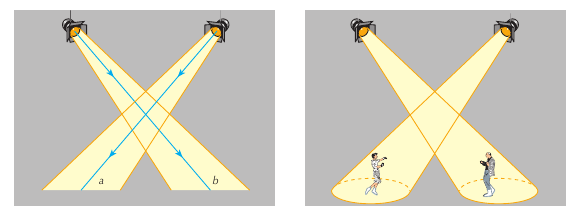
\includegraphics[width=2.5truein]{img16.png}
\caption{Independência dos raios. Fonte: Os Fundamentos da Física. Vol 2.}
\centering
\end{figure}

\begin{itemize}

\item \textbf{Princípio da reversibilidade da luz}:

\end{itemize}


A trajetória seguida pela luz não depende do seu sentido de percurso,


Ou seja, se a luz faz um determinado percurso, é capaz de fazer o mesmo percurso em sentido inverso.


\begin{figure}[h]{}
\centering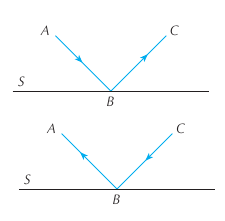
\includegraphics[width=2.5truein]{img17.png}
\caption{Reversibilidade. Fonte: Os Fundamentos da Física. Vol 2.}
\centering
\end{figure}

\hypertarget{x-sombra-e-penumbra}{\section{Sombra e penumbra}}
Primeiramente, vamos considerar um fonte puntiforme (\textbf{F}), um disco opaco (\textbf{D}) e um anteparo também opaco (\textbf{A}). Na montagem sugerida na figura, podemos perceber que, por causa da \textbf{propagação retilínea da luz}, teremos uma região desprovida de iluminação entre \textbf{D} e \textbf{A}, esta região (que é um tronco de cone) denominamos de \textbf{sombra}. Em \textbf{A} temos uma região circular também isenta de iluminação, que chamamos de \textbf{sombra projetada}.


\begin{figure}[h]{}
\centering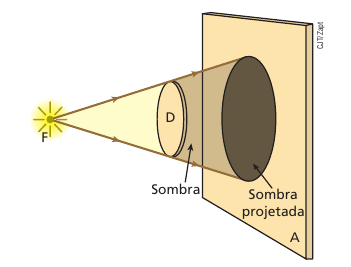
\includegraphics[width=2.5truein]{img18.png}
\caption{Sombra produzida por um fonte puntiforme. Fonte: Tópicos de Física. Vol 2.}
\centering
\end{figure}

Neste segundo caso, pelo fato da fonte de luz ser extensa, além das regiões de sombra e sombra projetada, teremos ainda regiões de \textbf{penumbra} e \textbf{penumbra projetada}. Nestas regiões a iluminação será \textbf{parcial}.


\begin{figure}[h]{}
\centering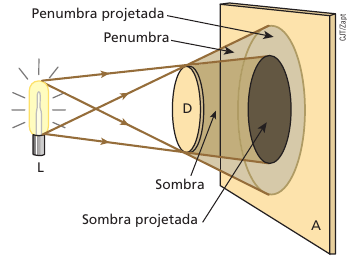
\includegraphics[width=2.5truein]{img19.png}
\caption{Sombra produzida por um fonte extensa. Fonte: Tópicos de Física. Vol 2.}
\centering
\end{figure}

\hypertarget{x-eclipse}{\subsection{Eclipse}}
Os eclipses são fenômenos astronômicos regulares e previsíveis. A explicação para a ocorrência dos eclipses está relacionada com a \textbf{propagação retilínea da luz}. É com base neste princípio que podemos explicar o desaparecimento temporário da Lua em certas ocasiões de lua cheia ou até mesmo do Sol, em algumas situações de lua Nova.


Podemos destacar dois casos.


1) \textbf{Eclipse da lua}: neste caso, a Lua situa-se no cone de sombra da Terra.


\begin{figure}[h]{}
\centering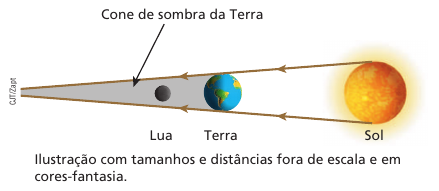
\includegraphics[width=2.5truein]{img20.png}
\caption{Eclipse da Lua. Fonte: Tópicos de Física. Vol 2.}
\centering
\end{figure}

O eclipse da Lua ocorre na fase de \textbf{lua cheia}.


1) \textbf{Eclipse do Sol}: neste caso, a Lua projeta sobre a Terra uma região de sombra e penumbra.


\begin{figure}[h]{}
\centering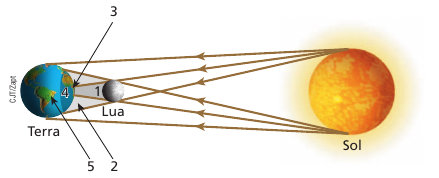
\includegraphics[width=2.5truein]{img21.png}
\caption{Eclipse do Sol. Fonte: Tópicos de Física. Vol 2.}
\centering
\end{figure}

\begin{itemize}

\item \textbf{Região 1}: sombra da Lua.

\item \textbf{Região 2}: penumbra.

\item \textbf{Região 3}: sombra da Lua projetada na Terra. Nesta região ocorre o eclipse total ou anular do Sol.

\item \textbf{Região 4}: penumbra projetada. Nesta região ocorre o elipse parcial do Sol, caso em que uma parte do "disco solar" permanece visível.

\item \textbf{Região 5}: não há eclipse nesta região. O "disco solar" é visualizado integralmente.

\end{itemize}


O eclipse da Sol ocorre na fase de \textbf{lua nova}.


\hypertarget{x-câmera-escura}{\subsection{Câmera escura}}
A \textbf{câmera escura} nada mais é que uma caixa de \textbf{paredes opacas}, sendo uma delas dotada de um orifício \textbf{$O$}, diante do qual é colocado um corpo luminoso.


Os raios emanados pelo corpo, após atravessarem o orifício \textbf{$O$}, incidem na parede ao fundo da caixa, projetando uma \textbf{imagem semelhante} ao corpo, porém \textbf{invertida}.


\begin{figure}[h]{}
\centering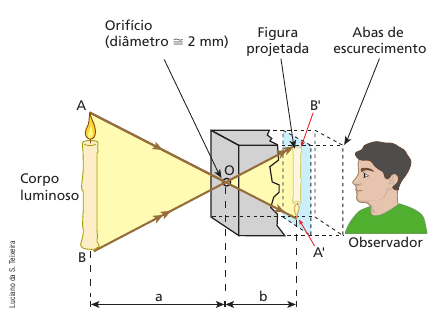
\includegraphics[width=2.5truein]{img22.png}
\caption{Câmera escura. Fonte: Tópicos de Física. Vol 2.}
\centering
\end{figure}

Considerando a figura, podemos notar que os triângulos $OAB$ e $OA'B'$ são semelhantes. Sendo assim:
\begin{equation*}
    \dfrac{A’B'}{AB}=\dfrac{b}{a}
\end{equation*}


Para uma mesma câmera e um mesmo corpo luminoso, os comprimentos \textbf{$b$} (profundidade) e \textbf{$AB$} (comprimento do corpo luminoso) são constantes. Desta forma, podemos afirmar que \textbf{$A'B'$} (comprimento da figura projetada) e \textbf{$a$} (distância do corpo luminoso ao orifício) são \textbf{inversamente proporcionais}. Por exemplo, se dobramos a distância \textbf{$A'B'$}, a distância \textbf{$a$} será reduzida pela metade.


\textbf{Exercício Resolvido 5}


\textbf{(UNIRIO RJ/1995)} Durante a final da Copa do Mundo, um cinegrafista, desejando alguns efeitos especiais, gravou cena em um estúdio completamente escuro, onde existia uma bandeira da "Azurra" (azul e branca) que foi iluminada por um feixe de luz amarela monocromática. Quando a cena foi exibida ao público, a bandeira apareceu:


a)	verde e branca. \\
b)	verde e amarela. \\
c)	preta e branca. \\
d)	preta e amarela. \\
e)	azul e branca.


\begin{resposta*}
{\it A cor azul absorve a luz monocromática amarela, portanto observamos o \textbf{preto.} A cor branca reflete a cor amarela, portanto continuamos a observar o \textbf{amarela}. \\
\textbf{Resposta: d.}}
\end{resposta*}

\textbf{Exercício Resolvido 6}


Marque \textbf{V} para verdadeiro e \textbf{F} para falso:


a) A formação de penumbra de um corpo opaco ocorre quando a fonte de luz é extensa. \\
b) O eclipse do Sol só ocorre numa fase de Lua Cheia e, portanto, todos os meses têm-se eclipses do Sol. \\
c) Quando ocorre eclipse do Sol a posição relativa dos três astros é Sol, Terra e Lua. \\
d) Uma pessoa na Terra se situa na penumbra da Lua determinada pelo Sol. Esta pessoa presencia um eclipse parcial do Sol. \\


\begin{resposta*}
{\it a) \textbf{Verdadeiro}. Quando uma fonte de luz extensa é colocada próxima de um corpo opaco observam-se regiões parcialmente iluminadas. São as penumbras. \\
b) \textbf{Falso}. No eclipse do Sol, a posição relativa dos astros é Sol, Lua e Terra. Portanto, o eclipse do Sol ocorre na fase de Lua Nova. Os eclipses não ocorrem todos os meses pois as órbitas da Lua em torno da Terra e da Terra em torno do Sol não pertencem ao mesmo plano. Os eclipses ocorrem quando a orbita da Lua intercepta o plano da órbita da Terra e ainda deve haver um alinhamento entre os três astros. \\
c) \textbf{Falso}. A posição relativa dos astros é Sol, Lua e Terra. \\
d) \textbf{Verdadeiro}. Estando na penumbra da Lua determinada pelo Sol o eclipse é parcial. \\}
\end{resposta*}

\textbf{Exercício Resolvido 7}


Entre uma fonte puntiforme e uma parede, coloca-se um lápis de $20\;cm$ de altura. A fonte de luz e o centro do lápis estão numa mesma reta perpendicular à parede. O lápis se encontra a $20\;cm$ da fonte e a $60\;cm$ da parede. Determine o comprimento da sombra do lápis projetada na parede.


\begin{figure}[h]{}
\centering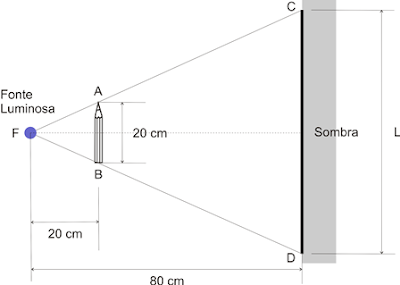
\includegraphics[width=2.5truein]{imgexe1.png}
\caption{Resolução. Fonte: blog osfundamentosdafisica. Vol 2.}
\centering
\end{figure}

\begin{resposta*}
{\it Da semelhança dos triângulos $FAB$ e $FCD$, temos:
\begin{align*}
    \dfrac{L}{20} &= \dfrac{80}{20} \\
    L &= 80
\end{align*}
\textbf{Resposta}: $80\;cm$.}
\end{resposta*}

\textbf{Exercício Resolvido 8}


Um objeto $AB$ de altura $10\;cm$ encontra-se a $30\;cm$ de uma câmara escura de orifício, cujo comprimento é de $45\;cm$.


a) Qual é a altura da imagem? \\
b) Aproxima-se o objeto da câmara. A altura da imagem aumenta ou diminui?


\begin{figure}[h]{}
\centering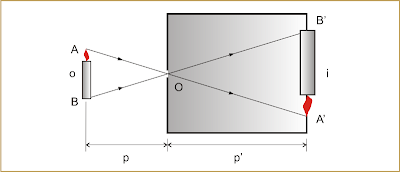
\includegraphics[width=2.5truein]{imgexe2.png}
\caption{Resolução. Fonte: blog osfundamentosdafisica. Vol 2.}
\centering
\end{figure}

\begin{resposta*}
{\it a)\textbf{Dados}: $o=10\;cm$ $p=30\;cm$ $p'=23\;cm$ \\
Pela semelhança de triângulos:
\begin{align*}
    \dfrac{i}{o}    &= \dfrac{p'}{p} \\
    i               &= o\cdot \dfrac{p}{p'} \\
    i               &= 10\cdot \dfrac{45}{30} \\
    i               &= 15
\end{align*}
\textbf{Resposta}: $15\;cm$. \\
b) Aproximando-se o objeto da câmara o valor de $p$ diminui e portanto a altura $i$ da imagem aumenta.}
\end{resposta*}

\textbf{Exercício de Revisão 5}


\textbf{(Mackenzie SP/2006)} Os objetos A e B, quando iluminados pela luz solar, apresentam, respectivamente, as cores vermelha e branca. Esses objetos, ao serem iluminados somente pela luz de uma lâmpada de sódio, que emite apenas a luz monocromática amarela, serão vistos, respectivamente, com as cores:


a)	vermelha e branca. \\
b)	laranja e amarela. \\
c)	vermelha e preta. \\
d)	preta e amarela. \\
e)	branca e preta.


\begin{resposta*}
{\it \textbf{d}.}
\end{resposta*}

\textbf{Exercício de Revisão 6}


\textbf{(UFT TO/2014)} Na década de 1980, a fibra óptica disseminou-se como um condutor de sinais em telecomunicações (telefones, televisão e redes de computadores). Menos de vinte anos depois, já existiam instalados, só nos Estados Unidos, cerca de 3.000.000 km de fibras ópticas. Elas são feitas de forma que um raio de luz, ao penetrar por uma de suas extremidades, não possa emergir pelas laterais devido ao fenômeno físico de:


a)	difração da luz. \\
b)	interferência da luz. \\
c)	reflexão da luz. \\
d)	propagação retilínea da luz. \\
e)	velocidade constante da luz.


\begin{resposta*}
{\it \textbf{c}.}
\end{resposta*}

\textbf{Exercício de Revisão 7}


\textbf{(UEPB/2006)} Um cineasta que trabalha com ficção científica, desenvolve um filme que trata da existência de um “novo universo”, em que um de seus planetas é iluminado com luz visível monocromática.  Considerando os diversos fenômenos ópticos causados por esta luz, pode-se afirmar que neste planeta não é possível observar:


a)	a formação da sombra \\
b)	a refração da luz \\
c)	a reflexão da luz \\
d)	um arco-íris \\
e)	a difração


\begin{resposta*}
{\it \textbf{d}.}
\end{resposta*}

\textbf{Exercício de Revisão 8}


\textbf{(ESCS DF/2010)} Um homem tem $1,80\;m$ de altura. A relação entre os tamanhos das imagens formadas numa câmara escura através de um orifício, quando o indivíduo se encontra, respectivamente, às distâncias de $48\;m$ e $72\;m$ será de:


a)	$3,5$ \\
b)	$3,0$ \\
c)	$2,5$ \\
d)	$2,0$ \\
e)	$1,5$


\begin{resposta*}
{\it \textbf{e}.}
\end{resposta*}

\textbf{Exercício de Revisão 9}


\textbf{(PUC RJ/2013)} A uma certa hora da manhã, a inclinação dos raios solares é tal que um muro de $4,0\;m$ de altura projeta, no chão horizontal, uma sombra de comprimento $6,0\;m$. Uma senhora de $1,6\;m$ de altura, caminhando na direção do muro, é totalmente coberta pela sombra quando se encontra a quantos metros do muro?


a)	$2,0$ \\
b)	$2,4$ \\
c)	$1,5$ \\
d)	$3,6$ \\
e)	$1,1$ \\


\begin{resposta*}
{\it \textbf{d}.}
\end{resposta*}

\textbf{Exercício de Revisão 10}


\textbf{(PUC SP/2014)} Em 15 de abril de 2014 ocorreu um eclipse lunar total que foi visível na parte oeste da África, na parte oeste da Europa, na parte leste da Ásia, nas Américas e na Austrália. Os eclipses totais da Lua, quando o satélite cruza o cone de sombra da Terra, são pouco frequentes. O último ocorreu no dia 10 de dezembro de 2011. Há ocorrência de tal eclipse.


a)	independentemente da fase da Lua, bastando, para isso, o alinhamento entre o Sol, a Lua e a Terra, nessa ordem. \\
b)	na lua nova. \\
c)	na lua cheia. \\
d)	no quarto crescente. \\
e)	no quarto minguante. \\


\begin{resposta*}
{\it \textbf{c}.}
\end{resposta*}

\hypertarget{x-referências}{\section{Referências}}
CALÇADA, Caio Sérgio; SAMPAIO, José Luiz. Física Clássica: Termologia, Óptica e Ondas. Atual Editora, São Paulo, 2012.


FERRARO, Nicolau Gilbert. "Óptica". Blog Os Fundamentos da Física. Disponível em: \href{https://osfundamentosdafisica.blogspot.com/}{https://osfundamentosdafisica.blogspot.com/}


RAMALHO JR, Francisco; FERRARO, Nicolau Gilberto; SOARES, Paulo Antônio de Toledo. Os Fundamentos da Física vol. 2. \textbf{Moderna, São Paulo}, 2007.


VILLAS BÔAS, Newton; DOCA, Ricardo Helou; BISCUOLA, Gualter José. Tópicos de física, 2: termologia, ondulatória e óptica. \textbf{São Paulo: Saraiva}, 2012.


\end{document}

